\documentclass[a4paper,12pt]{article}
\usepackage[a4paper, margin=2.5cm]{geometry}
\usepackage[pdftex]{graphicx}
\usepackage{tikz}
\usepackage{pgfplots}
\usepackage{enumitem}
\usepackage{float}
\usepackage[document]{ragged2e}
\usepackage[utf8]{inputenc}
\usepackage[T1]{fontenc}
\usepackage[spanish,es-tabla]{babel}
\renewcommand{\shorthandsspanish}{}
\usepackage{xurl}
\usepackage{lipsum}
\usepackage{mwe}
\usepackage{multicol}
\usepackage{siunitx}
\usepackage{listings}
\usepackage{enumitem}
\usepackage{amsmath}
\usepackage{listings}
\usepackage{tabularray}
\usepackage{schemata}
\usepackage{hyperref}


\graphicspath{ {/home/saikkopat/Documents/ESCOM/FiEmp/Proyecto-1} }

\begin{document}

\begin{titlepage}
	\begin{tikzpicture}[overlay, remember picture]
		\path (current page.north east) ++(-0.3,-1.8) node[below left] {
\includegraphics[width=0.35\textwidth]{/home/saikkopat/Documents/LOGOS IPN/EscudoESCOM}};
	\end{tikzpicture}
	\begin{tikzpicture}[overlay, remember picture]
		\path (current page.north west) ++(1.5,-1) node[below right] {
\includegraphics[width=0.2\textwidth]{/home/saikkopat/Documents/LOGOS IPN/logo}};
	\end{tikzpicture}
	\begin{center}
		\vspace{-1.5cm}
		{\LARGE Instituto Politécnico Nacional\par}
		\vspace{.5cm}
		{\LARGE Escuela Superior de Cómputo\par}
		\vspace{2.5cm}
		{\large Unidad de aprendizaje:}\\{\Large Finanzas empresariales\par}
		\vspace{5cm}
		{\scshape\Huge Proyecto\par}
		{\itshape\Large Primera etapa: análisis financiero de dos empresas\par}
		\vfill
		{\Large Integrantes:\par}
		\vspace{0.7cm}
		{\Large Gómez Tovar Yoshua Oziel\par}
		{\Large Boleta: 2023630391\par}
		\vspace{0.5cm}
		{\Large González Cárdenas Ángel Aquilez\par}
		{\Large Boleta: 2016630152\par}
		\vspace{0.5cm}
		{\Large Zarco Sosa Kevin\par}
		{\Large Boleta: 2023630735\par}
		\vspace{1cm}
		{\Large Grupo: 3CV4\par}
		\vspace{1cm}
		{\Large Profesor: Estrada Elizalde Serafín\par}
		\vfill
	\end{center}
\end{titlepage} 

\newpage

\tableofcontents

\newpage


\section{Introducción}

El presente documento detalla la información analisada para el desarrollo del proyecto del analisis finaciero de dos empresas perteneciente a la unidad de aprendizaje \emph{Finanzas Empresariales}.

\section{Objetivos}
En el desarrollo del presente documento que evidencia la conclusion de la primera parte del proyecto se contemplaron los siguientes objetivos:

\begin{enumerate}
	\item Historia de la creación, giro, evolución de la empresa a la actualidad.
	\item Misión, visión, eslogan.
	\item Mercado al que se dirige (perfil de sus clientes), y competidores principales.
	\item Organigrama
	\item Funcionamiento de la empresa en su actividad productiva y administrativa.
	\item Cuentas de Activos y pasivos que maneja y explicar cómo se componen.
\end{enumerate}

\clearpage

\section{Presentación de las Empresas}

\subsection{Historia de la creación de las empresas}

El mundo del calzado deportivo ha sido testigo de la creación y evolución de algunas de las marcas más icónicas y exitosas de la historia. Dos nombres que destacan en este universo son Nike y adidas. Detrás de estas gigantes corporaciones se encuentran historias fascinantes de determinación, innovación y visión empresarial.\par

En 1964, tras un viaje a Japón en el que conoció la firma de tenis Tiger, Knight decidió abrir junto a su entrenador de atletismo en la Universidad de Oregón la marca entonces llamada \emph{Blue Ribbon Sports}. Invirtieron 500 dólares cada uno y colaboraron con la casa japonesa para importar calzado a Estados Unidos. Siete años después, Knight fundaría Nike, compañía que factura ahora miles de millones de dólares.\par

Pagó entonces 35 dólares a la estudiante de diseño Carolyn Davidson para realizar un logotipo para su marca. El swoosh se convertiría en uno de los símbolos más reconocibles del mundo. Nike pasó de facturar 8,000 dólares en su primer año a cotizar en bolsa en los años 80. \par

El 18 de agosto de 1949, Adi Dassler fundó adidas, sin embargo, los inicios de la famosa compañía de calzado se remontan a 1924 cuado Adolf Dassler comenzó a fabricar calzado en Herzogenaurach, Alemania, después de su regreso de la Primera Guerra Mundial. Más tarde, su hermano mayor Rudolf se unió al negocio y se convirtió en la Fábrica de Zapatos de los Hermanos Dassler (Gebrüder Dassler Schuhfabrik). \par

La compañía Dassler promovió entonces el desarrollo de los zapatos para correr con púas para usarse en múltiples eventos deportivos. Para mejorar la calidad de este calzado, se impulsó la transición del modelo anterior de clavos de metal pesado a un modelo de lona y goma.\par

Ya en 1936, Dassler persuadió al velocista estadounidense, Jesse Owens, para usar su calzado de pico hechas a mano en los Juegos Olímpicos de Verano de 1936. Después de las cuatro medallas de oro de Owens, el nombre y la reputación de los zapatos Dassler se hicieron conocidos por los deportistas del mundo y sus entrenadores. Los hermanos ya vendían 200.000 pares de zapatos cada año antes de la Segunda Guerra Mundial.\par

Así, estas dos empresas, Nike y adidas, surgieron de raíces modestas y se convirtieron en gigantes globales en la industria del calzado deportivo. En este análisis financiero, exploraremos sus trayectorias, éxitos y desafíos a lo largo de los años, y compararemos sus logros financieros para comprender mejor el impacto que han tenido en el mundo empresarial y deportivo.\par

\subsection{Giro de las empresas}

Adidas y Nike son dos de las principales empresas en la industria del calzado deportivo y la ropa deportiva, y operan en el sector económico conocido como "Industria de Artículos Deportivos y Ropa Deportiva". Aunque ambas compañías se centran en la fabricación y venta de productos deportivos, tienen giros específicos y estrategias que las diferencian en este sector. De manera que los principales son:

Para \emph{Adidas}:
\begin{enumerate}
	\item Calzado Deportivo: Adidas es conocida por su amplia gama de calzado deportivo de alto rendimiento, diseñadas para deportes específicos como fútbol, baloncesto, correr y más.

	\item Ropa Deportiva: Además del calzado, Adidas fabrica y vende ropa deportiva, que incluye camisetas, pantalones, chaquetas y accesorios para una variedad de deportes y actividades físicas.

	\item Productos de Moda: Adidas ha desarrollado líneas de productos de moda y estilo de vida que combinan elementos deportivos con diseño urbano. Estos productos a menudo son populares en la cultura de la moda y el estilo callejero.

	\item Equipos Deportivos: La compañía también produce uniformes y equipos deportivos para equipos y atletas profesionales, universitarios y amateurs en varios deportes.

	\item Patrocinio Deportivo: Adidas es conocida por asociarse con atletas de renombre y equipos deportivos en todo el mundo como parte de su estrategia de marketing y patrocinio.
\end{enumerate}

Y por otra parte, para \emph{Nike}:
\begin{enumerate}
	\item Calzado Deportivo: Nike es famosa por su amplia línea de calzado deportivo está diseñado para una variedad de deportes, incluyendo el baloncesto, el fútbol, el atletismo y más. Su calzado icónico incluyen las Air Jordan y las Air Max.

	\item Ropa Deportiva: Al igual que Adidas, Nike produce una amplia gama de ropa deportiva, desde camisetas y pantalones hasta chaquetas y ropa de entrenamiento.

	\item Equipos y Accesorios: Nike fabrica y vende equipos deportivos, como balones de fútbol y baloncesto, así como accesorios deportivos como mochilas, calcetines y gorras.

	\item Tecnología Deportiva: Nike ha invertido en tecnología deportiva, como Nike+ y Nike Adapt, que integran la tecnología en el calzado deportivo para mejorar el rendimiento y la comodidad.

	\item Patrocinio Deportivo: Al igual que Adidas, Nike es conocida por sus patrocinios de atletas, equipos y eventos deportivos a nivel mundial, lo que la convierte en una de las marcas más reconocidas en el mundo del deporte.
\end{enumerate}

De este modo, Adidas y Nike operan en el mismo sector económico, pero tienen giros y estrategias ligeramente diferentes dentro de la industria de artículos deportivos y ropa deportiva. Ambas compañías son líderes en la industria y compiten activamente por cuota de mercado y reconocimiento de marca en todo el mundo.\par

\subsection{Evolución de las empresas en la actualidad}

Ambas empresas, Adidas y Nike, han experimentado una notable evolución a lo largo de las décadas, y la innovación ha sido una parte integral de su éxito continuo en la industria de artículos deportivos y ropa deportiva.

Por un lado, Adidas comenzó como una empresa centrada en el rendimiento deportivo, con un enfoque inicial en la fabricación de calzado de alto rendimiento para atletas. Su énfasis en la calidad y la innovación en el diseño de calzado la convirtió en una opción popular para deportistas. \par
Luego, a lo largo de los años, Adidas diversificó su enfoque para incluir la moda y el estilo de vida. Desarrollaron productos que no solo eran funcionales para el deporte, sino que también tenían un atractivo de moda, lo que les permitió llegar a un público más amplio. Adidas ha invertido en tecnología y materiales innovadores para mejorar el rendimiento de sus productos. Esto incluye la introducción de tecnologías como Boost en su calzado para una mayor comodidad y respuesta. \par

Por otra parte, Nike se ha destacado por su continua innovación en el diseño de calzado deportivo. Desde el lanzamiento de las icónicas Air Max hasta las tecnologías más recientes como Nike React y Nike Adapt, la empresa ha mantenido un enfoque constante en la mejora de la experiencia del usuario.
Nike ha sido pionera en el uso del marketing y el patrocinio deportivo como herramientas para construir su marca. Su asociación con atletas de renombre mundial y equipos deportivos ha sido fundamental para su éxito.
También ha integrado la tecnología en sus productos, desde aplicaciones de seguimiento de la actividad física hasta sistemas se autoajuste en su calzado. Esto ha permitido a la marca mantenerse relevante y atraer a un público más tecnológicamente orientado. \par

En resumen, tanto Adidas como Nike han evolucionado desde sus inicios como fabricantes de calzado deportivo de alto rendimiento hasta marcas globales que abarcan el rendimiento deportivo, la moda y la tecnología. La innovación ha sido un elemento clave en su capacidad para mantenerse en la cima de la industria, ya sea a través de avances en diseño de productos o por el uso de estrategias de marketing creativo. Ambas empresas han demostrado una capacidad constante para adaptarse a las tendencias cambiantes y hacer más que satisfacer las demandas de los consumidores.\par

\clearpage
\section{Mision de las empresas}

\subsection{Mision de Adidas}
\begin{quotation}
	El Grupo Adidas se esfuerza por ser el líder mundial en la industria de los artículos deportivos con marcas construidas sobre la pasión por deportes y un estilo de vida deportivo. Estamos comprometidos a fortalecer continuamente nuestras marcas y productos para mejorar nuestra posición competitiva
\end{quotation}
\subsection{Vision de Adidas}
\begin{quotation}
	Ser los líderes del diseño con un enfoque en obtener lo mejor de los atletas con productos de rendimiento garantizado en el mercado deportivo a nivel mundial.
\end{quotation}
\subsection{Eslogan de Adidas}
Adidas ha utilizado varios esloganes a lo largo de su historia. Uno de los esloganes más conocidos y duraderos de Adidas es:
\begin{quotation}
	Impossible is nothing
\end{quotation}


\subsection{Mision de Nike}
\begin{quotation}
	Llevar la inspiración y la innovación a cada atleta del mundo.
\end{quotation}
\subsection{Vision de Nike}
\begin{quotation}
	Trabajar constantemente para expandir su impacto positivo en el mundo y ser la empresa líder en la industria de artículos deportivos y ropa deportiva. Nike aspira a ser una marca que inspire a las personas a moverse y vivir activamente.
\end{quotation}
\subsection{Eslogan de Nike}
El eslogan más icónico y reconocible de Nike es: 
\begin{quotation}
	Just Do It
\end{quotation}


\clearpage
\section{Perfilamiento en el mercado y competidores}

\subsection{Participacion en el mercado}

De Bejarano y Polanco, tenemos los siguientes comentarios:

\begin{quotation}
	Para el 2013, Adidas es la segunda marca más reconocida, junto a Reebok
(también propiedad de Adidas). Adidas es considerado como una marca que se
relaciona con todos los aspectos de la moda, la ropa y del uso de sus productos
en cualquier circunstancia. Gracias al cambio de identidad de Adidas, ahora es
vista como una marca dinámica. Adidas maneja sus propios valores, que busca
que sean asociados a su concepto de marca: el rendimiento, la autenticidad, la
honestidad, la sinceridad, el compromiso e igualdad.
\end{quotation}
Y, por otra parte:
\begin{quotation}
	Nike orienta su producción hacía varias categorías claves como: Atletismo,
Baloncesto, Fútbol, el acondicionamiento tanto de hombres como mujeres, Nike
Sports wear y Action Sports. También comercializa productos deportivos para el
béisbol, Cricket, Golf, Lacrosse, actividades al aire libre, fútbol americano, tenis,
voleibol, y para la lucha libre. Así mismo tiene una línea de productos para los
niños. El calzado deportivo de Nike está diseñado principalmente para un deporte
en específico. Niketambién ofrece bolsos, maletines, calcetines, balones de
deporte, gafas, relojes, aparatos electrónicos, bates, guantes, equipo de
protección, palos de golf y otros equipos diseñados para las actividades
deportivas.
\end{quotation}

De este modo, tenemos que Nike quiere representar el nivel de servicio más alto dentro y fuera
de su industria, construyen relaciones con los consumidores de todo el mundo
basadas en la lealtadm promocionando sus productos mediante acuerdos de
patrocinio con atletas famosos, con equipos profesionales y con equipos
deportivos universitarios.\par
En contraste, tiliza la personalidad de los jugadores de fútbol más
reconocidos en la actualidad para transmitir todos los rasgos y cualidades del sus
productos, así el consumidor cuando está en el proceso de compra, se siente más
cerca de ser como el modelo actual de la marca. Por ejemplo, David Beckhames
un modelo a seguir para muchos; cuando el consumidor se viste con los productos
de Adidas, se siente más cerca de ser como él, es decir se atribuye, por medio del
uso de dichos productos, las cualidades de Beckham: puede llegar a sentirse
sexy, triunfador, bello, superado, caballeroso, empático, agresivo, luchador,
exitoso o que tiene el mejor desempeño.\par

\clearpage
\subsection{Competidores}

Por un lado, los principales competidores de Adidas son:
\begin{itemize}
\item \textbf{Puma}: Otra marca reconocida a nivel global que compite directamente con Adidas.
\item \textbf{Converse}: Conocida principalmente por sus icónicos zapatos deportivos Chuck Taylor All Star.
\item \textbf{Vans}: Una marca de calzado y ropa que se ha vuelto especialmente popular en la cultura del skateboarding y la moda urbana.
\item \textbf{Reebok}: Adquirida por Adidas en 2005, es una marca que ha mantenido su propia identidad y compite directamente con Adidas en muchos aspectos.
\item \textbf{New Balance}: Una empresa estadounidense que se ha destacado en la fabricación de calzado deportivo, ropa y accesorios.
\end{itemize}

Por otra parte, los principales competidores de Nike son:
\begin{itemize}
\item \textbf{Reebok}: Con ingresos mundiales de \$3 mil millones y una valoración de marca de \$1 mil millones, Reebok es considerado el segundo mayor competidor de Nike en todo el mundo.
\item \textbf{Puma}: Con ingresos de \$3.4 mil millones, Puma es el tercer competidor de Nike.
\end{itemize}

\clearpage

\section{Organigrama}

Adidas presenta una estructura jerárquica vertical de tres niveles. A la cabeza de la pirámide está el Consejo de Administración compuesto por los accionistas. Sus miembros se llaman Consejeros y entre ellos se pueden distribuir los cargos de Presidente, Vicepresidente, Secretario y Consejero delegado. En la misma línea descendente aparece la figura de la Gerencia quien se encarga del Control de la Gestión y de la administración de la entidad.

En el siguiente nivel del organigrama aparecen seis departamentos.

\begin{itemize}
	\item \textbf{Producción} que se encarga de todo el proceso productivo de la empresa, la transformación y planificación.

\item \textbf{Administración y Finanzas} se encarga de los proveedores, clientes cobros y pagos. Entran entre sus funciones la contabilidad financiera de la entidad, costos y negocios bancarios.
\item \textbf{Marketing} se encarga de las estrategias del mercado, políticas de precio, distribución y comunicación. Es responsable de la imagen de la empresa.
\item \textbf{Comercial y ventas} se encarga de todo lo relativo a la cartera de clientes y la captación de los nuevos.
\item \textbf{Compras} se encarga de la negociación con los proveedores, los pedidos y gestión de almacén.
\item \textbf{Área de Calidad} aparece en un tercer nivel en relación estrecha con los departamentos de Compras y Producción. Se encarga del control de calidad y laboratorio.
\item \textbf{Recursos Humanos} se encarga de la selección del personal, nóminas y relación con los sindicatos.
\end{itemize}

\begin{figure}[ht!]
	\centering

	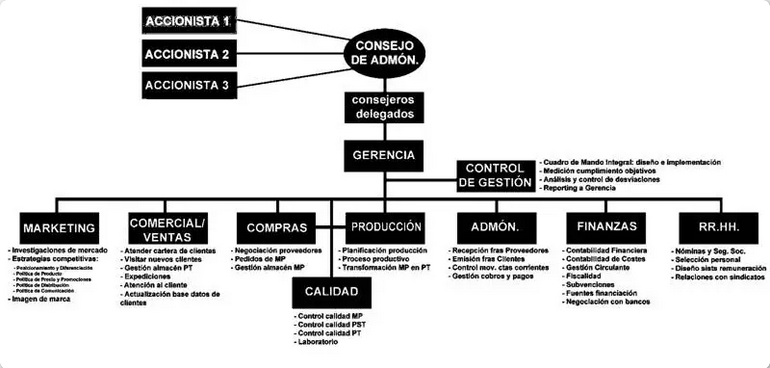
\includegraphics[width=.9\textwidth]{adi}

	\caption{Organigrama de Adidas}
\end{figure}


\clearpage
Por otra parte, Nike tiene una matriz estructura organizativa incorporando divisiones geográficas. La estructura matricial de Nike también está presente a nivel regional y subregional. La responsabilidad gerencial se segmenta de acuerdo con la unidad de negocios (ropa, calzado y equipo) y la función (recursos humanos, finanzas, Marketing, ventas y operaciones).

\begin{figure}[ht!]
	\centering

	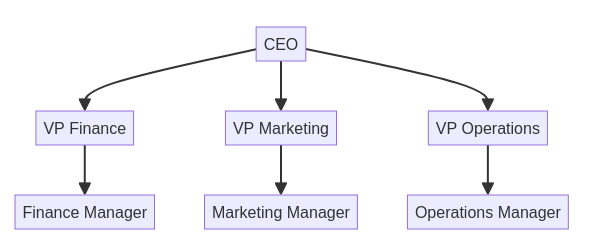
\includegraphics[width=.75\textwidth]{nike}

	\caption{Organigrama matricial de Nike}
\end{figure}

\section{Funcionamiento de la empresa en su actividad productiva y administrativa.}
Tanto Nike como Adidas son empresas líderes en la industria de artículos deportivos y ropa deportiva que han demostrado su capacidad para operar de manera eficiente en la actividad productiva y administrativa. Su compromiso con la innovación, la calidad, la sostenibilidad y el marketing efectivo los ha llevado a mantener su posición de liderazgo en un mercado altamente competitivo.

\subsection{Actividad Productiva de Nike}

\textbf{Investigación y Desarrollo (I+D):} Nike es conocida por su compromiso con la innovación en el diseño y la fabricación de productos deportivos. Invierte significativamente en investigación y desarrollo para crear tecnologías y materiales avanzados que mejoren el rendimiento de sus productos.

\textbf{Fabricación Global:} Nike produce sus productos en todo el mundo a través de una extensa red de proveedores y fábricas. Esto le permite diversificar su producción y mantener una respuesta ágil a la demanda en todo el mundo.

\textbf{Personalización y Personalización:} Nike ofrece a los clientes la opción de personalizar productos como zapatillas de deporte a través de su plataforma Nike By You. Esto no solo brinda una experiencia de compra personalizada, sino que también contribuye a la lealtad de los clientes.

\textbf{Sostenibilidad:} Nike ha intensificado sus esfuerzos en sostenibilidad, utilizando materiales reciclados y aplicando prácticas sostenibles en la fabricación de productos. También se ha comprometido a reducir su huella de carbono.

\subsection{Actividad Administrativa de Nike}

\textbf{Gestión de la Cadena de Suministro:} Nike tiene un enfoque riguroso en la gestión de la cadena de suministro para garantizar la disponibilidad de productos en todo el mundo. Esto incluye la planificación de la demanda y la logística eficiente.

\textbf{Marketing y Patrocinio:} Nike es conocida por su estrategia de marketing efectiva y su asociación con atletas de renombre y equipos deportivos. Estas asociaciones y campañas publicitarias contribuyen significativamente a su presencia global.

\subsection{Actividad Productiva de Adidas}

\textbf{Diseño de Producto:} Adidas se enfoca en el diseño de productos atractivos y funcionales. Trabaja en colaboración con atletas y diseñadores para crear artículos deportivos de alta calidad.

\textbf{Sostenibilidad:} Adidas también ha hecho hincapié en la sostenibilidad, utilizando materiales reciclados y adoptando prácticas responsables en la fabricación de productos.

\subsection{Actividad Administrativa de Adidas}

\textbf{Estrategia de Marketing:} Adidas ha implementado estrategias de marketing creativas y colaboraciones con celebridades y diseñadores para mantener su atractivo en el mercado de la moda deportiva.

\textbf{Gestión de Marca:} La marca Adidas es cuidadosamente gestionada, manteniendo una imagen de calidad y estilo que resuena con los consumidores.



\clearpage

\section{Cuentas de Activos y pasivos}

Los activos son los recursos económicos que posee una empresa, como el efectivo, las cuentas por cobrar, las inversiones a corto plazo, etc. Estos pueden ser convertidos en efectivo o se espera que proporcionen un beneficio en el futuro.

Los pasivos son las obligaciones financieras o deudas que la empresa debe pagar a otras entidades. Pueden incluir cuentas por pagar, préstamos, salarios por pagar, etc.

El análisis de estas cuentas puede proporcionar información valiosa sobre la salud financiera de una empresa.

Cabe señalar que el patrimonio de los accionistas incluye elementos como acción ordinaria, ganancias acumuladas y otro resultado integral acumulado. Estos representan los recursos propios de la empresa, incluyendo las inversiones de los accionistas y las ganancias acumuladas a lo largo del tiempo.

Las siguientes tablas proporcionan una vista desglosada de los activos, pasivos y el patrimonio de los accionistas de la empresa en tres años consecutivos. Esto permite realizar un seguimiento de cómo han evolucionado estos elementos a lo largo del tiempo y proporciona información importante para el análisis financiero y la toma de decisiones.


\subsection{Balance general de Adidas}

\begin{figure}[ht!]
	\centering

	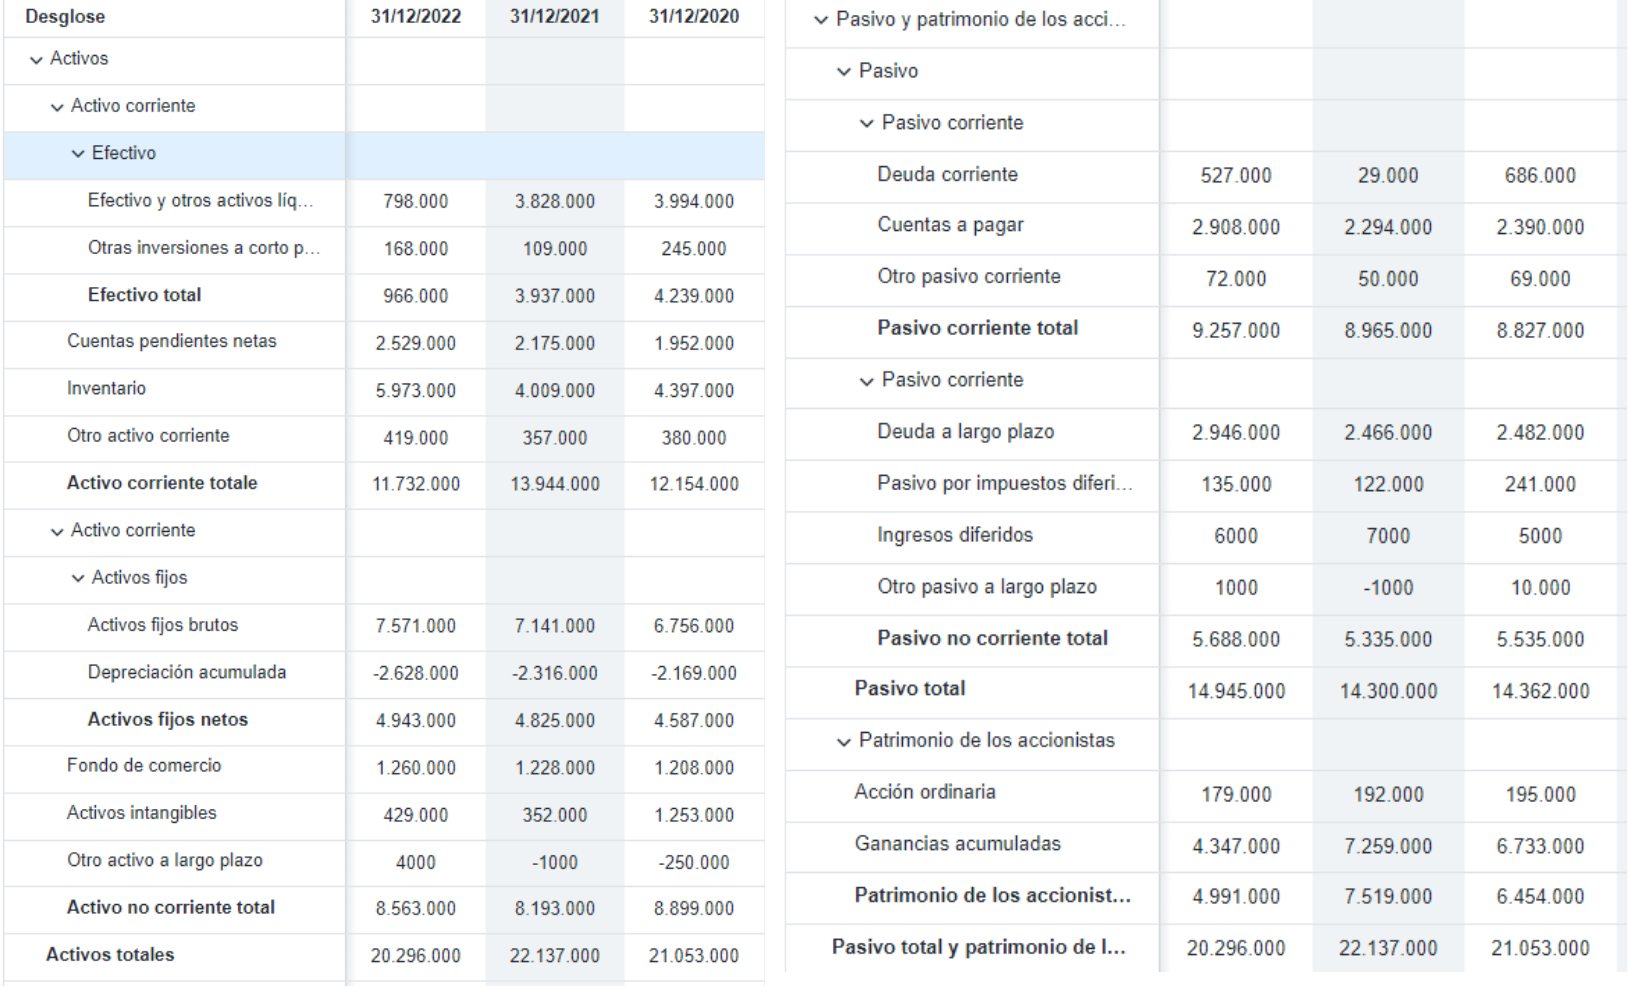
\includegraphics[width=.9\textwidth]{AdidasB}
\end{figure}

\begin{figure}[ht!]
	\centering

	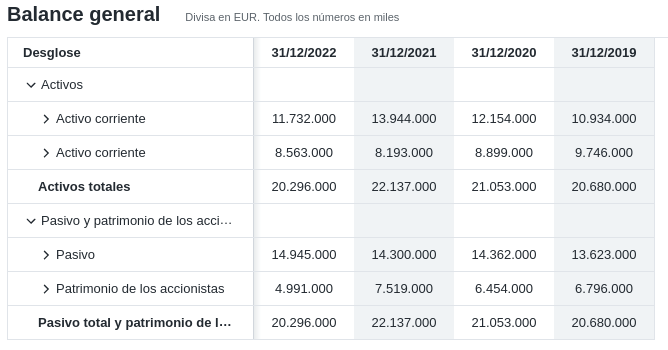
\includegraphics[width=.9\textwidth]{AdidasBA}
\end{figure}


Esta tabla presenta un desglose de los activos de la empresa, pero para los años 2020, 2021 y 2022.
Se divide en dos secciones principales: activo corriente y activos fijos.
El activo corriente incluye categorías como efectivo y otros activos líquidos, cuentas pendientes netas, inventario y otros activos corrientes.
En esta tabla, se observa una disminución significativa en la cantidad de efectivo en comparación con los años anteriores. También se observa un aumento en las cuentas pendientes netas y en el inventario.
Los activos fijos incluyen activos como activos fijos brutos, depreciación acumulada, activos fijos netos, fondo de comercio, activos intangibles y otros activos a largo plazo.
Se observa que el fondo de comercio y los activos intangibles han experimentado cambios en sus valores.

Por otro lado tabla presenta un desglose del pasivo y el patrimonio de los accionistas de la empresa, también para los años 2020, 2021 y 2022.
Se divide en tres secciones principales: pasivo corriente, pasivo no corriente y patrimonio de los accionistas.
El pasivo corriente incluye categorías como deuda corriente, cuentas a pagar, otro pasivo corriente y pasivo corriente total. Se observa un aumento en la deuda corriente y cuentas a pagar en comparación con los años anteriores.
El pasivo no corriente incluye categorías como deuda a largo plazo, pasivo por impuestos diferidos, ingresos diferidos y otro pasivo a largo plazo. Se observan cambios en los valores de estas categorías.
El patrimonio de los accionistas incluye elementos como acción ordinaria y ganancias acumuladas. Se observa una disminución en las ganancias acumuladas en el año 2022 en comparación con el año anterior.

Se pueden identificar cambios significativos en los activos, pasivos y el patrimonio de los accionistas, lo que pudo ser relevante para el análisis financiero y la toma de decisiones.



\clearpage
\subsection{Balance general de Nike}

\begin{figure}[ht!]
	\centering

	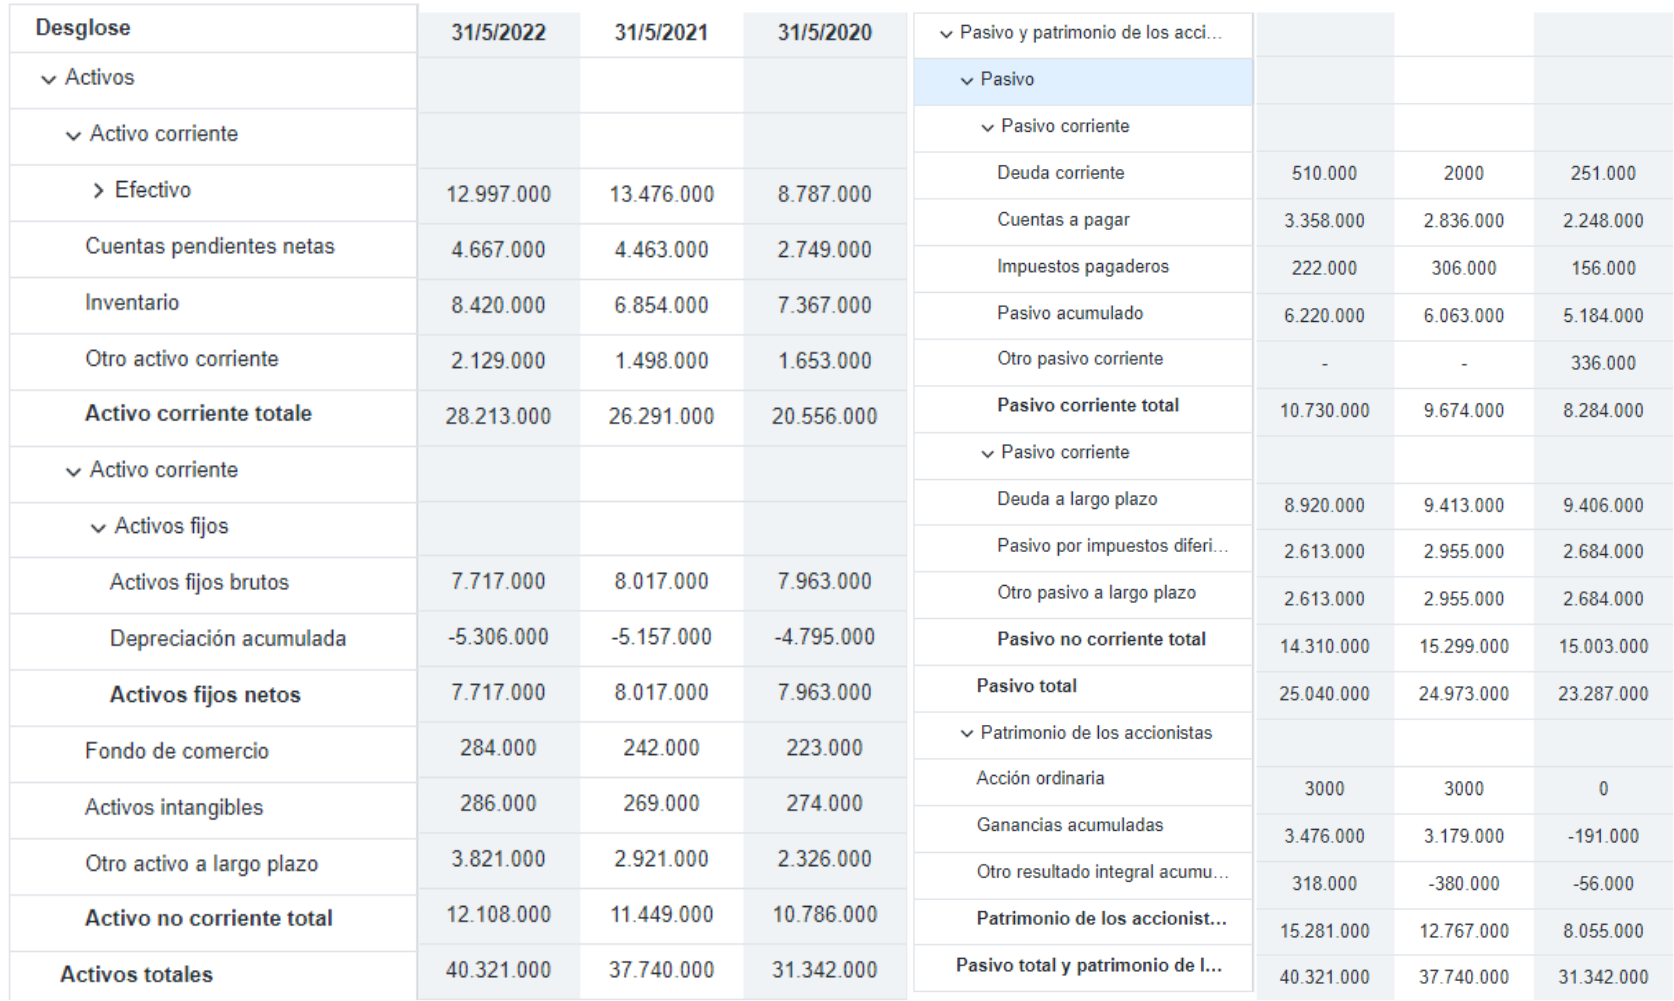
\includegraphics[width=.9\textwidth]{NikeB}
\end{figure}

\begin{figure}[ht!]
	\centering

	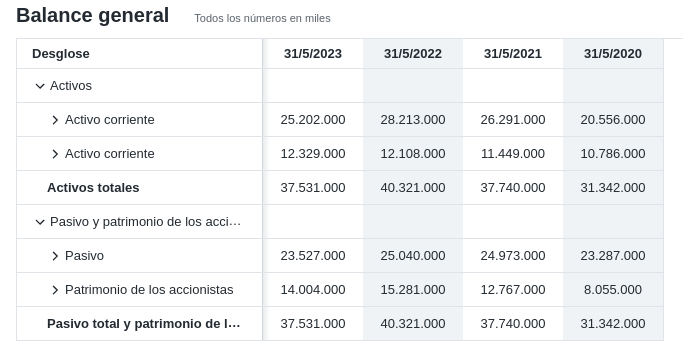
\includegraphics[width=.9\textwidth]{NikeBA}
\end{figure}

Del balance para Nike tenemos que se presenta un desglose de los activos de la empresa para los años 2020, 2021 y 2022.
Se divide en dos secciones principales: activo corriente y activos fijos.
El activo corriente incluye categorías como efectivo, cuentas pendientes netas, inventario y otros activos corrientes. Estos representan los activos que se espera que se conviertan en efectivo o se utilicen en el corto plazo.
Los activos fijos incluyen activos como activos fijos brutos, depreciación acumulada, activos fijos netos, fondo de comercio, activos intangibles y otros activos a largo plazo. Estos representan activos a largo plazo que no se espera que se conviertan en efectivo en el corto plazo.


En esta tabla, se presenta un desglose del pasivo y el patrimonio de los accionistas de la empresa para los años 2020, 2021 y 2022.
Se divide en tres secciones principales: pasivo corriente, pasivo no corriente y patrimonio de los accionistas.
El pasivo corriente incluye categorías como deuda corriente, cuentas a pagar, impuestos pagaderos, pasivo acumulado y otros pasivos corrientes. Estos representan las obligaciones de la empresa que se espera que se paguen en el corto plazo.
El pasivo no corriente incluye categorías como deuda a largo plazo, pasivo por impuestos diferidos y otros pasivos a largo plazo. Estos representan las obligaciones de la empresa a largo plazo.



\clearpage
\section{Anexos}

\subsection{Anexo: Organigrama Adidas}

\begin{figure}[ht!]
	\centering

	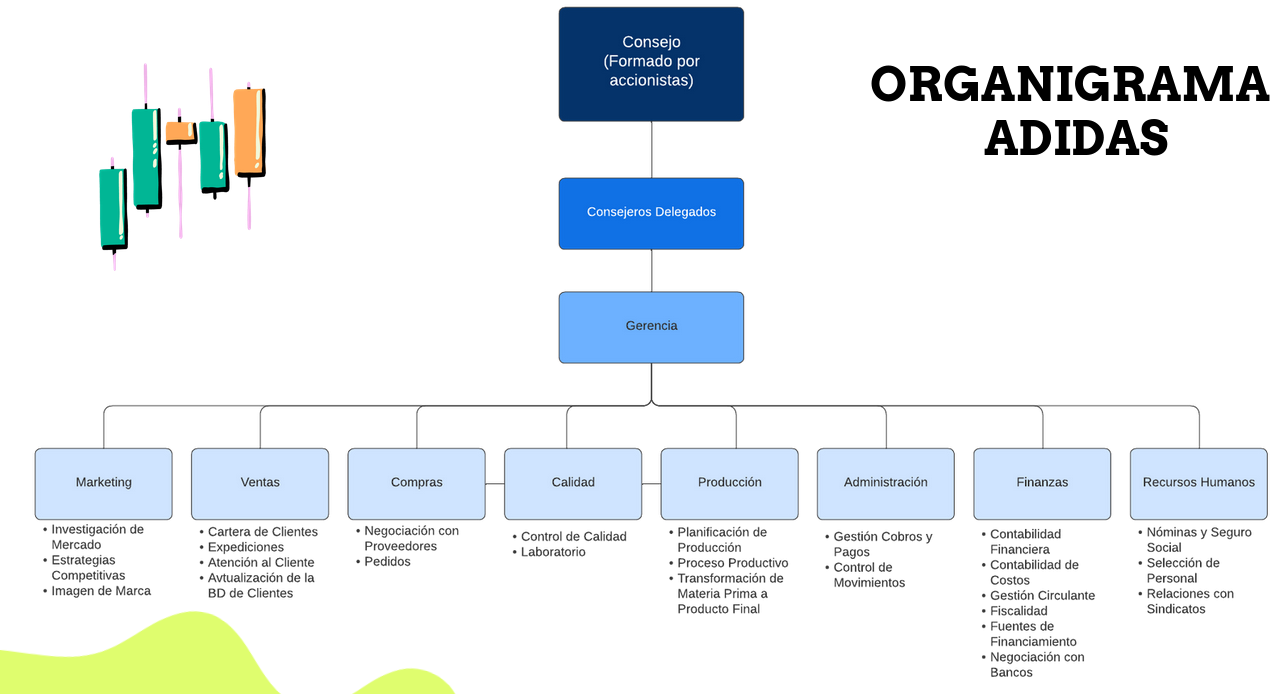
\includegraphics[width=.9\textwidth]{OAdidas}
\end{figure}

\subsection{Anexo: Organigrama Nike}

\begin{figure}[ht!]
	\centering

	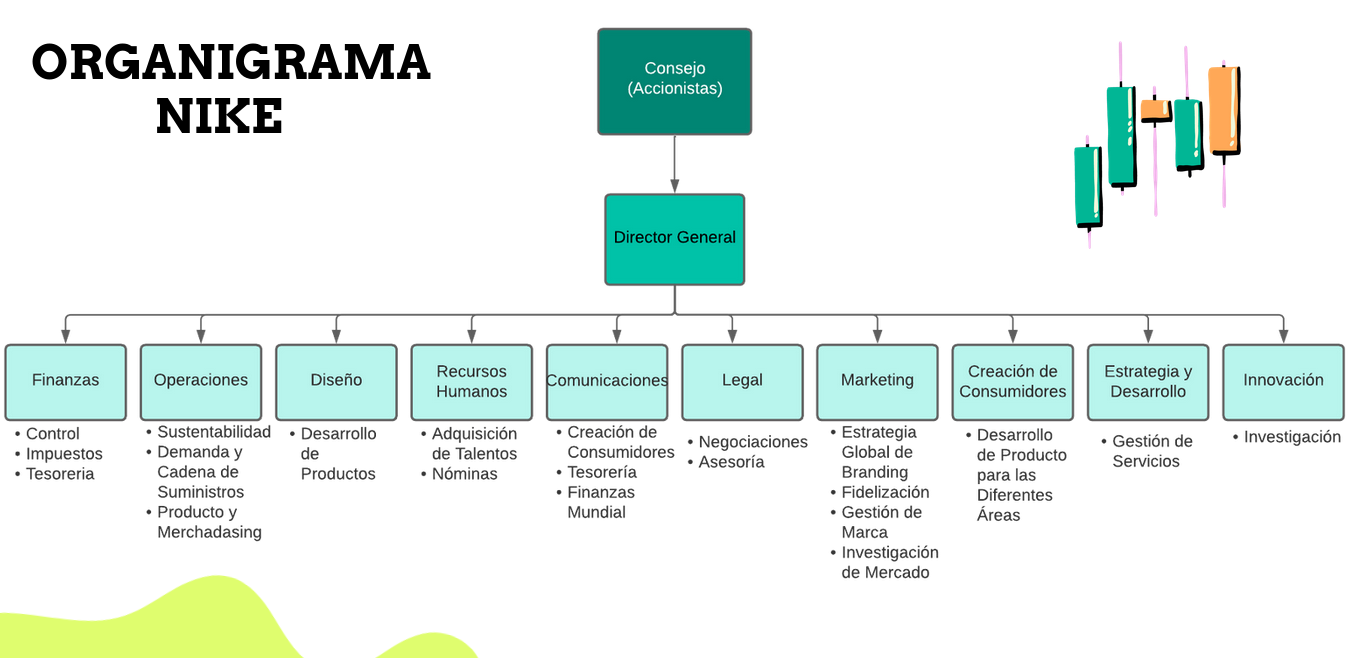
\includegraphics[width=.9\textwidth]{ONike}
\end{figure}

\clearpage

\section{Referencias}
\begin{enumerate}
\item \textit{Balance General de Adidas (ADSN) - Investing.com México.} (s/f). Investing.com México. Recuperado el 3 de octubre de 2023, de \url{https://mx.investing.com/equities/adidas-salomon-balance-sheet?cid=993700}
\item \textit{Balance General de Nike (NKE) - Investing.com México.} (s/f). Investing.com México. Recuperado el 3 de octubre de 2023, de \url{https://mx.investing.com/equities/nike-balance-sheet?cid=993836}
\item Hernández, E. (2023, febrero 24). \textit{La historia de cómo sólo 500 dólares se necesitaron para fundar Nike.} Forbes México. \url{https://www.forbes.com.mx/la-historia-de-como-solo-500-dolares-se-necesitaron-para-fundar-nike/}
\item \textit{Los 10 mejores competidores de Nike - Marketing e Influencer.} (2022, agosto 21). cruzito. \url{https://marketingeinfluencer.com/los-10-mejores-competidores-de-nike/}
\item \textit{Organigrama de Adidas.} (2022, junio 1). Organigramas. \url{https://organigramadeunaempresa.info/adidas/}
\item Oyarzún, G. (2023, mayo 4). \textit{El origen de la marca Adidas: historia, evolución y estrategia comercial.} EspacioEmpresa. \url{https://espacioempresa.com/lideres/adidas-origen/}
\item (S/f-a). Mission-statement.com. Recuperado el 3 de octubre de 2023, de \url{https://mission-statement.com/adidas-es/}
\item (S/f-b). Mission-statement.com. Recuperado el 3 de octubre de 2023, de \url{https://mission-statement.com/nike-es/}
\item (S/f-c). Edu.co. Recuperado el 3 de octubre de 2023, de \url{https://repository.icesi.edu.co/biblioteca_digital/bitstream/10906/78628/1/TG01013.pdf}
1.5: Cuentas de Activos, Pasivos y Accionistas. (2022, October 30). LibreTexts Español; Libretexts. \url{https://espanol.libretexts.org/Negocio/Contabilidad/Libro%3A_Principios_de_Contabilidad_Financiera_(Jonick)/01%3A_Ciclo_Contable_para_el_Negocio_de_Servicios_-_Base_de_Efectivo/1.05%3A_Cuentas_de_Activos%2C_Pasivos_y_Accionistas}

\item adidas AG (ADDYY). (s.f.). Yahoo.com. Recuperado el 4 de octubre de 2023, de \url{https://es.finance.yahoo.com/quote/ADDYY/balance-sheet/?guccounter=1}

\item NIKE, Inc. (NKE). (s.f.). Yahoo.com. Recuperado el 4 de octubre de 2023, de \url{https://es.finance.yahoo.com/quote/NKE/balance-sheet/}

\end{enumerate}



\end{document}